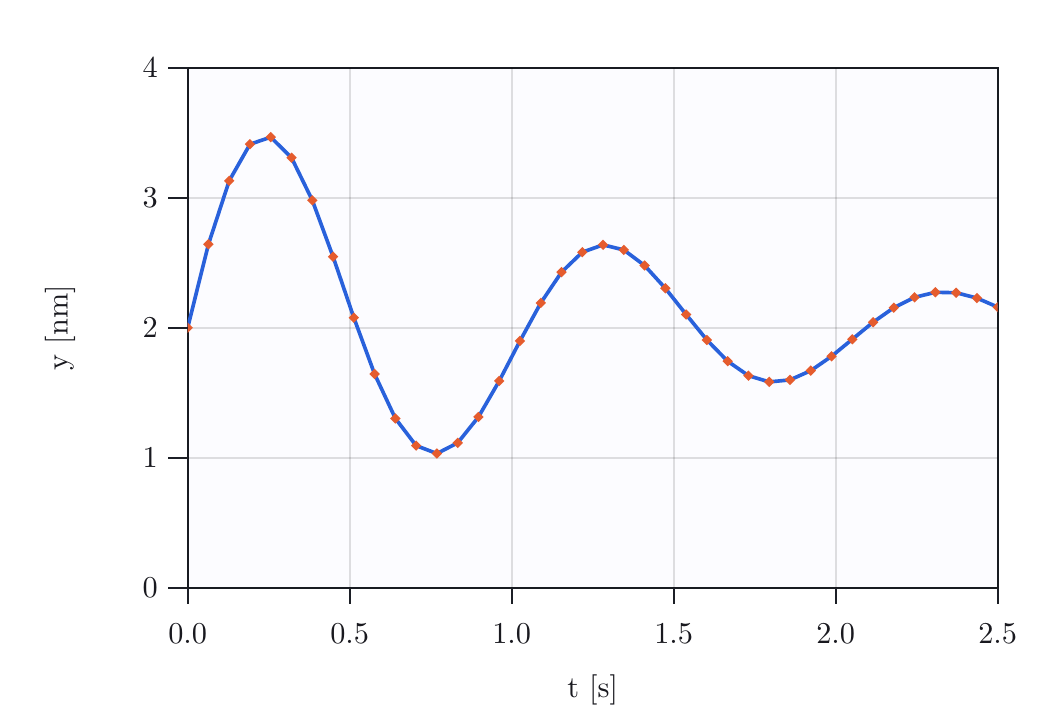
\begin{tikzpicture}[every node/.style={inner sep=0bp,outer sep=0bp}]
  \definecolor{qcA}{rgb}{0.99,0.99,1}
  \definecolor{qcB}{rgb}{0.11,0.12,0.15}
  \definecolor{qcC}{rgb}{0,0,0}
  \definecolor{qcD}{rgb}{0.16,0.38,0.86}
  \def\quivermarkE#1#2{\path[fill,shift={(#1,#2)}] (0bp,-1.875bp) -- (1.875bp,0bp) -- (0bp,1.875bp) -- (-1.875bp,0bp) -- cycle;}
  \definecolor{qcF}{rgb}{0.9,0.36,0.18}
  \definecolor{qcG}{rgb}{0.1,0.1,0.12}
  \useasboundingbox (0bp,0bp) rectangle (360bp,240bp);
  % quiver-key: figure
  \path[fill=qcA,draw=qcB,line width=0.75bp] (57.6bp,38.4bp) -- (349.2bp,38.4bp) -- (349.2bp,225.6bp) -- (57.6bp,225.6bp) -- cycle;
  % quiver-role: decoration
  \path[draw=qcC,draw opacity=0.12,line width=0.75bp] (57.6bp,38.4bp) -- (57.6bp,225.6bp);
  \path[draw=qcC,draw opacity=0.12,line width=0.75bp] (115.92bp,38.4bp) -- (115.92bp,225.6bp);
  \path[draw=qcC,draw opacity=0.12,line width=0.75bp] (174.24bp,38.4bp) -- (174.24bp,225.6bp);
  \path[draw=qcC,draw opacity=0.12,line width=0.75bp] (232.56bp,38.4bp) -- (232.56bp,225.6bp);
  \path[draw=qcC,draw opacity=0.12,line width=0.75bp] (290.88bp,38.4bp) -- (290.88bp,225.6bp);
  \path[draw=qcC,draw opacity=0.12,line width=0.75bp] (349.2bp,38.4bp) -- (349.2bp,225.6bp);
  \path[draw=qcC,draw opacity=0.12,line width=0.75bp] (57.6bp,38.4bp) -- (349.2bp,38.4bp);
  \path[draw=qcC,draw opacity=0.12,line width=0.75bp] (57.6bp,85.2bp) -- (349.2bp,85.2bp);
  \path[draw=qcC,draw opacity=0.12,line width=0.75bp] (57.6bp,132bp) -- (349.2bp,132bp);
  \path[draw=qcC,draw opacity=0.12,line width=0.75bp] (57.6bp,178.8bp) -- (349.2bp,178.8bp);
  \path[draw=qcC,draw opacity=0.12,line width=0.75bp] (57.6bp,225.6bp) -- (349.2bp,225.6bp);
  \begin{scope}
    \clip (57.6bp,38.4bp) -- (349.2bp,38.4bp) -- (349.2bp,225.6bp) -- (57.6bp,225.6bp) -- cycle;
    % quiver-role: series -- displacement
    % quiver-data: n = 40
    \path[draw=qcD,line width=1.313bp] (57.6bp,132bp) -- (65.077bp,162.027bp) -- (72.554bp,184.884bp) -- (80.031bp,198.04bp) -- (87.508bp,200.581bp) -- (94.985bp,193.184bp) -- (102.462bp,177.862bp) -- (109.938bp,157.552bp) -- (117.415bp,135.612bp) -- (124.892bp,115.3bp) -- (132.369bp,99.328bp) -- (139.846bp,89.53bp) -- (147.323bp,86.688bp) -- (154.8bp,90.526bp) -- (162.277bp,99.851bp) -- (169.754bp,112.81bp) -- (177.231bp,127.217bp) -- (184.708bp,140.896bp) -- (192.185bp,151.984bp) -- (199.662bp,159.168bp) -- (207.138bp,161.812bp) -- (214.615bp,159.986bp) -- (222.092bp,154.383bp) -- (229.569bp,146.163bp) -- (237.046bp,136.743bp) -- (244.523bp,127.572bp) -- (252bp,119.92bp) -- (259.477bp,114.721bp) -- (266.954bp,112.47bp) -- (274.431bp,113.199bp) -- (281.908bp,116.513bp) -- (289.385bp,121.693bp) -- (296.862bp,127.824bp) -- (304.338bp,133.948bp) -- (311.815bp,139.199bp) -- (319.292bp,142.922bp) -- (326.769bp,144.738bp) -- (334.246bp,144.577bp) -- (341.723bp,142.654bp) -- (349.2bp,139.414bp);
    \begin{scope}[fill=qcF]
      \quivermarkE{57.6bp}{132bp}
      \quivermarkE{65.077bp}{162.027bp}
      \quivermarkE{72.554bp}{184.884bp}
      \quivermarkE{80.031bp}{198.04bp}
      \quivermarkE{87.508bp}{200.581bp}
      \quivermarkE{94.985bp}{193.184bp}
      \quivermarkE{102.462bp}{177.862bp}
      \quivermarkE{109.938bp}{157.552bp}
      \quivermarkE{117.415bp}{135.612bp}
      \quivermarkE{124.892bp}{115.3bp}
      \quivermarkE{132.369bp}{99.328bp}
      \quivermarkE{139.846bp}{89.53bp}
      \quivermarkE{147.323bp}{86.688bp}
      \quivermarkE{154.8bp}{90.526bp}
      \quivermarkE{162.277bp}{99.851bp}
      \quivermarkE{169.754bp}{112.81bp}
      \quivermarkE{177.231bp}{127.217bp}
      \quivermarkE{184.708bp}{140.896bp}
      \quivermarkE{192.185bp}{151.984bp}
      \quivermarkE{199.662bp}{159.168bp}
      \quivermarkE{207.138bp}{161.812bp}
      \quivermarkE{214.615bp}{159.986bp}
      \quivermarkE{222.092bp}{154.383bp}
      \quivermarkE{229.569bp}{146.163bp}
      \quivermarkE{237.046bp}{136.743bp}
      \quivermarkE{244.523bp}{127.572bp}
      \quivermarkE{252bp}{119.92bp}
      \quivermarkE{259.477bp}{114.721bp}
      \quivermarkE{266.954bp}{112.47bp}
      \quivermarkE{274.431bp}{113.199bp}
      \quivermarkE{281.908bp}{116.513bp}
      \quivermarkE{289.385bp}{121.693bp}
      \quivermarkE{296.862bp}{127.824bp}
      \quivermarkE{304.338bp}{133.948bp}
      \quivermarkE{311.815bp}{139.199bp}
      \quivermarkE{319.292bp}{142.922bp}
      \quivermarkE{326.769bp}{144.738bp}
      \quivermarkE{334.246bp}{144.577bp}
      \quivermarkE{341.723bp}{142.654bp}
      \quivermarkE{349.2bp}{139.414bp}
    \end{scope}
  \end{scope}
  % quiver-role: axis -- t [s]
  % quiver-data: unit = s
  \path[draw=qcB,line width=0.75bp] (57.6bp,38.4bp) -- (57.6bp,32.4bp);
  \node[anchor=north,text=qcG,font=\fontsize{11}{13.2}\selectfont] at (57.6bp,25.2bp) {0.0};
  \path[draw=qcB,line width=0.75bp] (115.92bp,38.4bp) -- (115.92bp,32.4bp);
  \node[anchor=north,text=qcG,font=\fontsize{11}{13.2}\selectfont] at (115.92bp,25.2bp) {0.5};
  \path[draw=qcB,line width=0.75bp] (174.24bp,38.4bp) -- (174.24bp,32.4bp);
  \node[anchor=north,text=qcG,font=\fontsize{11}{13.2}\selectfont] at (174.24bp,25.2bp) {1.0};
  \path[draw=qcB,line width=0.75bp] (232.56bp,38.4bp) -- (232.56bp,32.4bp);
  \node[anchor=north,text=qcG,font=\fontsize{11}{13.2}\selectfont] at (232.56bp,25.2bp) {1.5};
  \path[draw=qcB,line width=0.75bp] (290.88bp,38.4bp) -- (290.88bp,32.4bp);
  \node[anchor=north,text=qcG,font=\fontsize{11}{13.2}\selectfont] at (290.88bp,25.2bp) {2.0};
  \path[draw=qcB,line width=0.75bp] (349.2bp,38.4bp) -- (349.2bp,32.4bp);
  \node[anchor=north,text=qcG,font=\fontsize{11}{13.2}\selectfont] at (349.2bp,25.2bp) {2.5};
  \node[anchor=north,text=qcG,font=\fontsize{11}{13.2}\selectfont] at (203.4bp,7.2bp) {t [s]};
  % quiver-role: axis -- y [nm]
  % quiver-data: unit = nm
  \path[draw=qcB,line width=0.75bp] (57.6bp,38.4bp) -- (50.4bp,38.4bp);
  \node[anchor=east,text=qcG,font=\fontsize{11}{13.2}\selectfont] at (46.8bp,38.4bp) {0};
  \path[draw=qcB,line width=0.75bp] (57.6bp,85.2bp) -- (50.4bp,85.2bp);
  \node[anchor=east,text=qcG,font=\fontsize{11}{13.2}\selectfont] at (46.8bp,85.2bp) {1};
  \path[draw=qcB,line width=0.75bp] (57.6bp,132bp) -- (50.4bp,132bp);
  \node[anchor=east,text=qcG,font=\fontsize{11}{13.2}\selectfont] at (46.8bp,132bp) {2};
  \path[draw=qcB,line width=0.75bp] (57.6bp,178.8bp) -- (50.4bp,178.8bp);
  \node[anchor=east,text=qcG,font=\fontsize{11}{13.2}\selectfont] at (46.8bp,178.8bp) {3};
  \path[draw=qcB,line width=0.75bp] (57.6bp,225.6bp) -- (50.4bp,225.6bp);
  \node[anchor=east,text=qcG,font=\fontsize{11}{13.2}\selectfont] at (46.8bp,225.6bp) {4};
  \node[anchor=base,text=qcG,rotate=90,font=\fontsize{11}{13.2}\selectfont] at (14.4bp,132bp) {y [nm]};
\end{tikzpicture}
